\documentclass[12pt]{article}
\usepackage[margin=2.5cm]{geometry}
\usepackage{graphicx}
\usepackage{amsmath}
\usepackage{float}
\usepackage{tikz}
\usepackage{pgfplots}

\linespread{1.0}

\begin{document}


	\noindent \textit{Philip Salmony, Wolfson College, pms67@cam.ac.uk} \hfill 15 January 2019

	\vspace{0.25cm}

	\begin{center}
		\hrule \vspace{0.3cm} \huge{\textbf{Technical Milestone Report}}  \\
		\Large{F-FF286-2: Self-Balancing Bike} \\
		\vspace{0.2cm}
		\hrule
	\end{center}
	
\vspace{0.2cm}	
	
\section{Introduction and Background}
This project involves the modelling, simulation, control system design, and implementation of a rider-less, self-balancing bicycle. Bicycles and their stability properties have been studied for well over a century, most notably by academics such as Whipple (1899 [1]), Papadopoulos (1980s onwards, [2]), and Astrom (2005, [3]). Most people know that a bicycle can be self-stable under certain conditions but it is still commonly unclear what primarily contributes to this self-stability. The equations of motion are tedious to understand intuitively, as they are a set of coupled and highly non-linear differential equations. \\

\noindent In addition to simply understanding the causes of self-stability of a bicycle, there are further interesting aims to studying a bicycle in the frameworks of dynamics and control theory. For example, how does a human stabilise a bicycle and can we replicate this behaviour with motors? What makes a bike more or less stable (such as changes in geometry, mass distribution, or wheel size - to name a few)? And would there be a benefit in having an 'assisted' bicycle for certain people in certain situations? \\

\noindent This project therefore aims to try and answer - at least in part - some of these questions, with a primary focus on achieving closed-loop stability under a large range of forward velocities. The bicycle only has a drive actuator, to provide forward velocity, and an actuator placed at the handlebars to provide a \textit{steer} torque. Without the additional component of being able to provide a \textit{lean} torque, it is extremely difficult to guarantee stability at near-zero forward speed as will be shown in this report. The bicycle being studied in this case can therefore be classed as an \textit{underactuated system}. \\

\noindent This report outlines the work completed so far and gives a plan regarding what work will be completed in Lent term.

\section{Previously Completed Work}
This section presents the work completed during the summer of 2018 and Michaelmas term 2018, including the completion of a functioning prototype self-balancing bicycle.

\subsection{Modelling}
Initially, to be able to investigate bicycle stability and ultimately design a stabilising controller for the system, it was necessary to model the dynamics of the bicycle.

\subsubsection{Equations of Motion}
As mentioned in the \textit{Introduction and Background} section, the differential equations governing the motion of a bicycle are highly non-linear and coupled. These equations of motion are far too complex to gain any useful intuition from and additionally make controller design difficult. \\

\noindent Therefore, it was decided to utilise simplified, linearised equations of motion. An initial linearised equation of motion, relating the \textit{steer} angle to the \textit{lean} angle of the bicycle, is of second order and does not take the bicycle front fork dynamics into account. Additionally taking the bicycle's front fork dynamics into account gives a set of coupled second order differential equation, resulting in an overall fourth-order system representation. This is typically given in the following form:

\begin{equation}
\mathbf{M} \cdot \underline{\ddot{q}} + \mathbf{C_1} \cdot v \cdot \underline{\dot{q}} + (\mathbf{K_0} + \mathbf{K_2} v^2) \cdot \underline{q} = \begin{bmatrix}
0 \\
\tau
\end{bmatrix}
\end{equation}

\vspace{0.2cm}

\noindent Where $\mathbf{M}$, $\mathbf{C_1}$, $\mathbf{K_0}$ and $\mathbf{K_2}$ are mass, damping, and stiffness matrices respectively, $\underline{q}$ is a column vector containing the lean angle ($\phi$) and steer angle ($\delta$), and $v$ is the forward velocity. $\tau$ is the handlebar torque. The equation is linearised about zero lean angle, however it is non-linear in forward velocity. \\

\noindent An excellent, far more elaborate discussion on bicycle dynamics used here as the basis for modelling is given in [3]. \\

\noindent As can be seen from the equations above, there is a \textit{strong} dependence on forward speed and is one of the main governors of overall stability. For a full-scale bicycle, a plot showing the real parts of the eigenvalues of the system versus forward speed is shown in \textit{Figure 1} below.

\begin{figure}[H]
	\begin{tikzpicture}
		\begin{axis}
			[xlabel=Forward Speed $v$,
			 ylabel=Real Part of Eigenvalue $\lambda$,
			 xmin=0,xmax=6,
			 ymin=-10,ymax=5]
			\addplot[mark=none] table[x=v,y=a, col sep=comma] {StabilityVsForwardSpeed.csv};
			\addplot[mark=none] table[x=v,y=b, col sep=comma] {StabilityVsForwardSpeed.csv};
			\addplot[mark=none] table[x=v,y=c, col sep=comma] {StabilityVsForwardSpeed.csv};
			\addplot[mark=none] table[x=v,y=d, col sep=comma] {StabilityVsForwardSpeed.csv};
			
			\draw [dashed, thin] (0,0) -- (6,0);
			\draw [dotted, thin] (3,-10) -- (3,5);
			\draw [dotted, thin] (4.8,-10) -- (4.8,5);
		\end{axis}
	\end{tikzpicture}
	\centering
	\caption{Pole Locations vs Forward Speed}
\end{figure}

\noindent As seen from the plot, the bicycle is increasingly unstable as it approaches zero forward velocity, self-stable between approximately $3$ and $4ms^{-1}$, and slightly unstable above this. \\

\noindent Therefore, a suitable controller must cope well with changes in forward speed.

\subsubsection{Estimation of System Parameters}
The equations of motion demand a knowledge of certain system parameters, such as inertia tensors and centers of mass. To calculate these, a Python script was written that uses finite element methods. In particular, the discretised forms of the moment of inertia and center of mass integrals were used over a quantised three-dimensional grid on which the basic bicycle frame, fork, and wheels were layed out.

\subsubsection{State-Space Model}
After having estimated the system parameters, these could then be combined with the equations of motion and transformed into a state-space representation. Two real-world bicycles were available: a Lego Mindstorms prototype, and a full-size adult bicycle.
For instance, for the full-scale bicycle, the state-space model dynamics ($\mathbf{A}$) and input ($\mathbf{B}$) matrices were found to be:

\begin{equation}
\mathbf{A} = \begin{bmatrix}
0 & 0 & 1 & 0 \\
0 & 0 & 0 & 1 \\
17 & 0.76 - 1.9v^2 & -0.51v & -1.1v \\
1.4 & 10-0.60v^2 & 5.1v & -1.3v
\end{bmatrix} \\
, \mathbf{B} = \begin{bmatrix}
0 & 0 & -0.57 & 5.8
\end{bmatrix}^T
\end{equation}

\noindent With the states being $\underline{x}=[\phi, \delta, \dot{\phi}, \dot{\delta}]$.

\subsection{Simulation}
After having investigated a set of suitable equations of motions for modelling and analysis, it was important to have tools to visualise the system and test the suitability of controllers before final implementation.

\subsubsection{Matlab}
Matlab in combination with Simulink was chosen as the basis for controller synthesis and analysis. Their use is demonstrated in section 2.3, \textit{Controller Design}.

\subsubsection{Unity}
Unity is an industry-standard 3D engine primarily used for computer games. A complete simulation environment was developed using this, to visualise the bicycle dynamics and controller effectiveness in a simulated 3D environment. Furthermore, various parameters could be tuned 'on-the-go' and in real-time, such as sensor noise, actuator saturation and delay, and forward speed which are obstacles encountered in the final, real-world implementation. The equations of motion were integrated using the Runge-Kutta fourth-order method and a discretised version of the designed controllers was implemented using the programming language C\#. Various initial conditions can be set, as well as impulse and steps fed as inputs to the system on command. A screenshot can be seen in \textit{Figure 2} below.
The full source code for this and the Python script can be found in [A].

\begin{figure}[H]
\centering
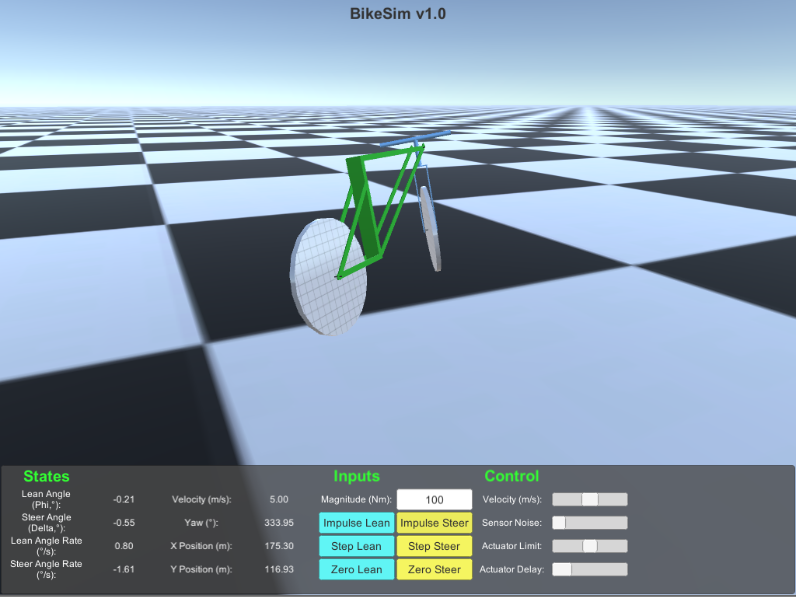
\includegraphics[scale=0.5]{BikeSim}
\caption{Screenshot of Unity Bike Simulator}
\end{figure}

\subsection{Controller Design}
Having suitable simulation environments then allowed the design of control algorithms with the aim of stabilising the bicycle in an upright position at ideally \textit{any} forward velocity. Broadly speaking, two classes of controller designs were investigated: linear and non-linear.

\subsubsection{Linear}
\textbf{Linear Quadratic Regulator} \\
Given the state-space model described above, a natural first choice was to try a full-state feedback approach, since all states are easily measurable on the real system and do not require an observer. Thus, an LQR controller was synthesized using Matlab's built-in function and then tested in Simulink. Theoretically, the LQR approach could stabilise the system at any forward velocity - albeit with extraordinarily large gains at near-zero velocity. This was however not taking into account hindrances such as actuator limits. Furthermore, any linear approach would need gain-scheduling to work anywhere close to satisfactorily during the final implementation, as stability varies drastically at different operating points (i.e. forward velocities). \\

\noindent \textbf{Proportional-Derivative} \\
Secondly, a more classical, single-loop controller design was investigated. Using primarily the root-locus method, proportional and derivative controller gains were chosen based on desired damping ratios and requirements for stability. Derivative action was needed to provide the necessary damping to maintain stability, as a proportional-only controller could never stabilise the bicycle. As before, theoretically it was seen that a controller could be synthesized that stabilised the bicycle at any operating point. Again, gain-scheduling would be needed.

\subsubsection{Non-Linear}
The desire to attain a \textit{single} control algorithm that works across the \textit{entire} range of forward velocities led on to the topic of non-linear controller design. Two strategies were suggested by my supervisor, Dr. Fulvio Forni: \textit{Virtual Model Control} [4] and \textit{Energy-Balancing Control} [5]. Both approaches work well and are intuitive for fairly simple systems. However, manipulating the bicycle system equations into the required form for both approaches proved challenging. However, a simple virtual model controller (using a virtual spring and virtual dashpot attached to the top of the bicycle frame) was found to work in simulation - across the entire range of forward velocities using just a single control strategy.

\subsection{Lego Mindstorms Prototype}
Using Lego Mindstorms and programmed using RobotC, a prototype bicycle was developed to test the previously simulated control algorithms. The prototype can be seen in \textit{Figure 3} below. Initially, only linear control strategies were tested. LQR-based control was not able to stabilise the prototype. PD control however \textit{was} able to stabilise the bicycle. However, the controller gains calculated using Matlab did not match the controller gains needed, which indicates some form of modelling error, which will be investigated further. Nonetheless, it is a promising success to have made a self-stabilising prototype by the end of Michaelmas term.
A video of the prototype can be seen in [B].

\begin{figure}[H]
\centering
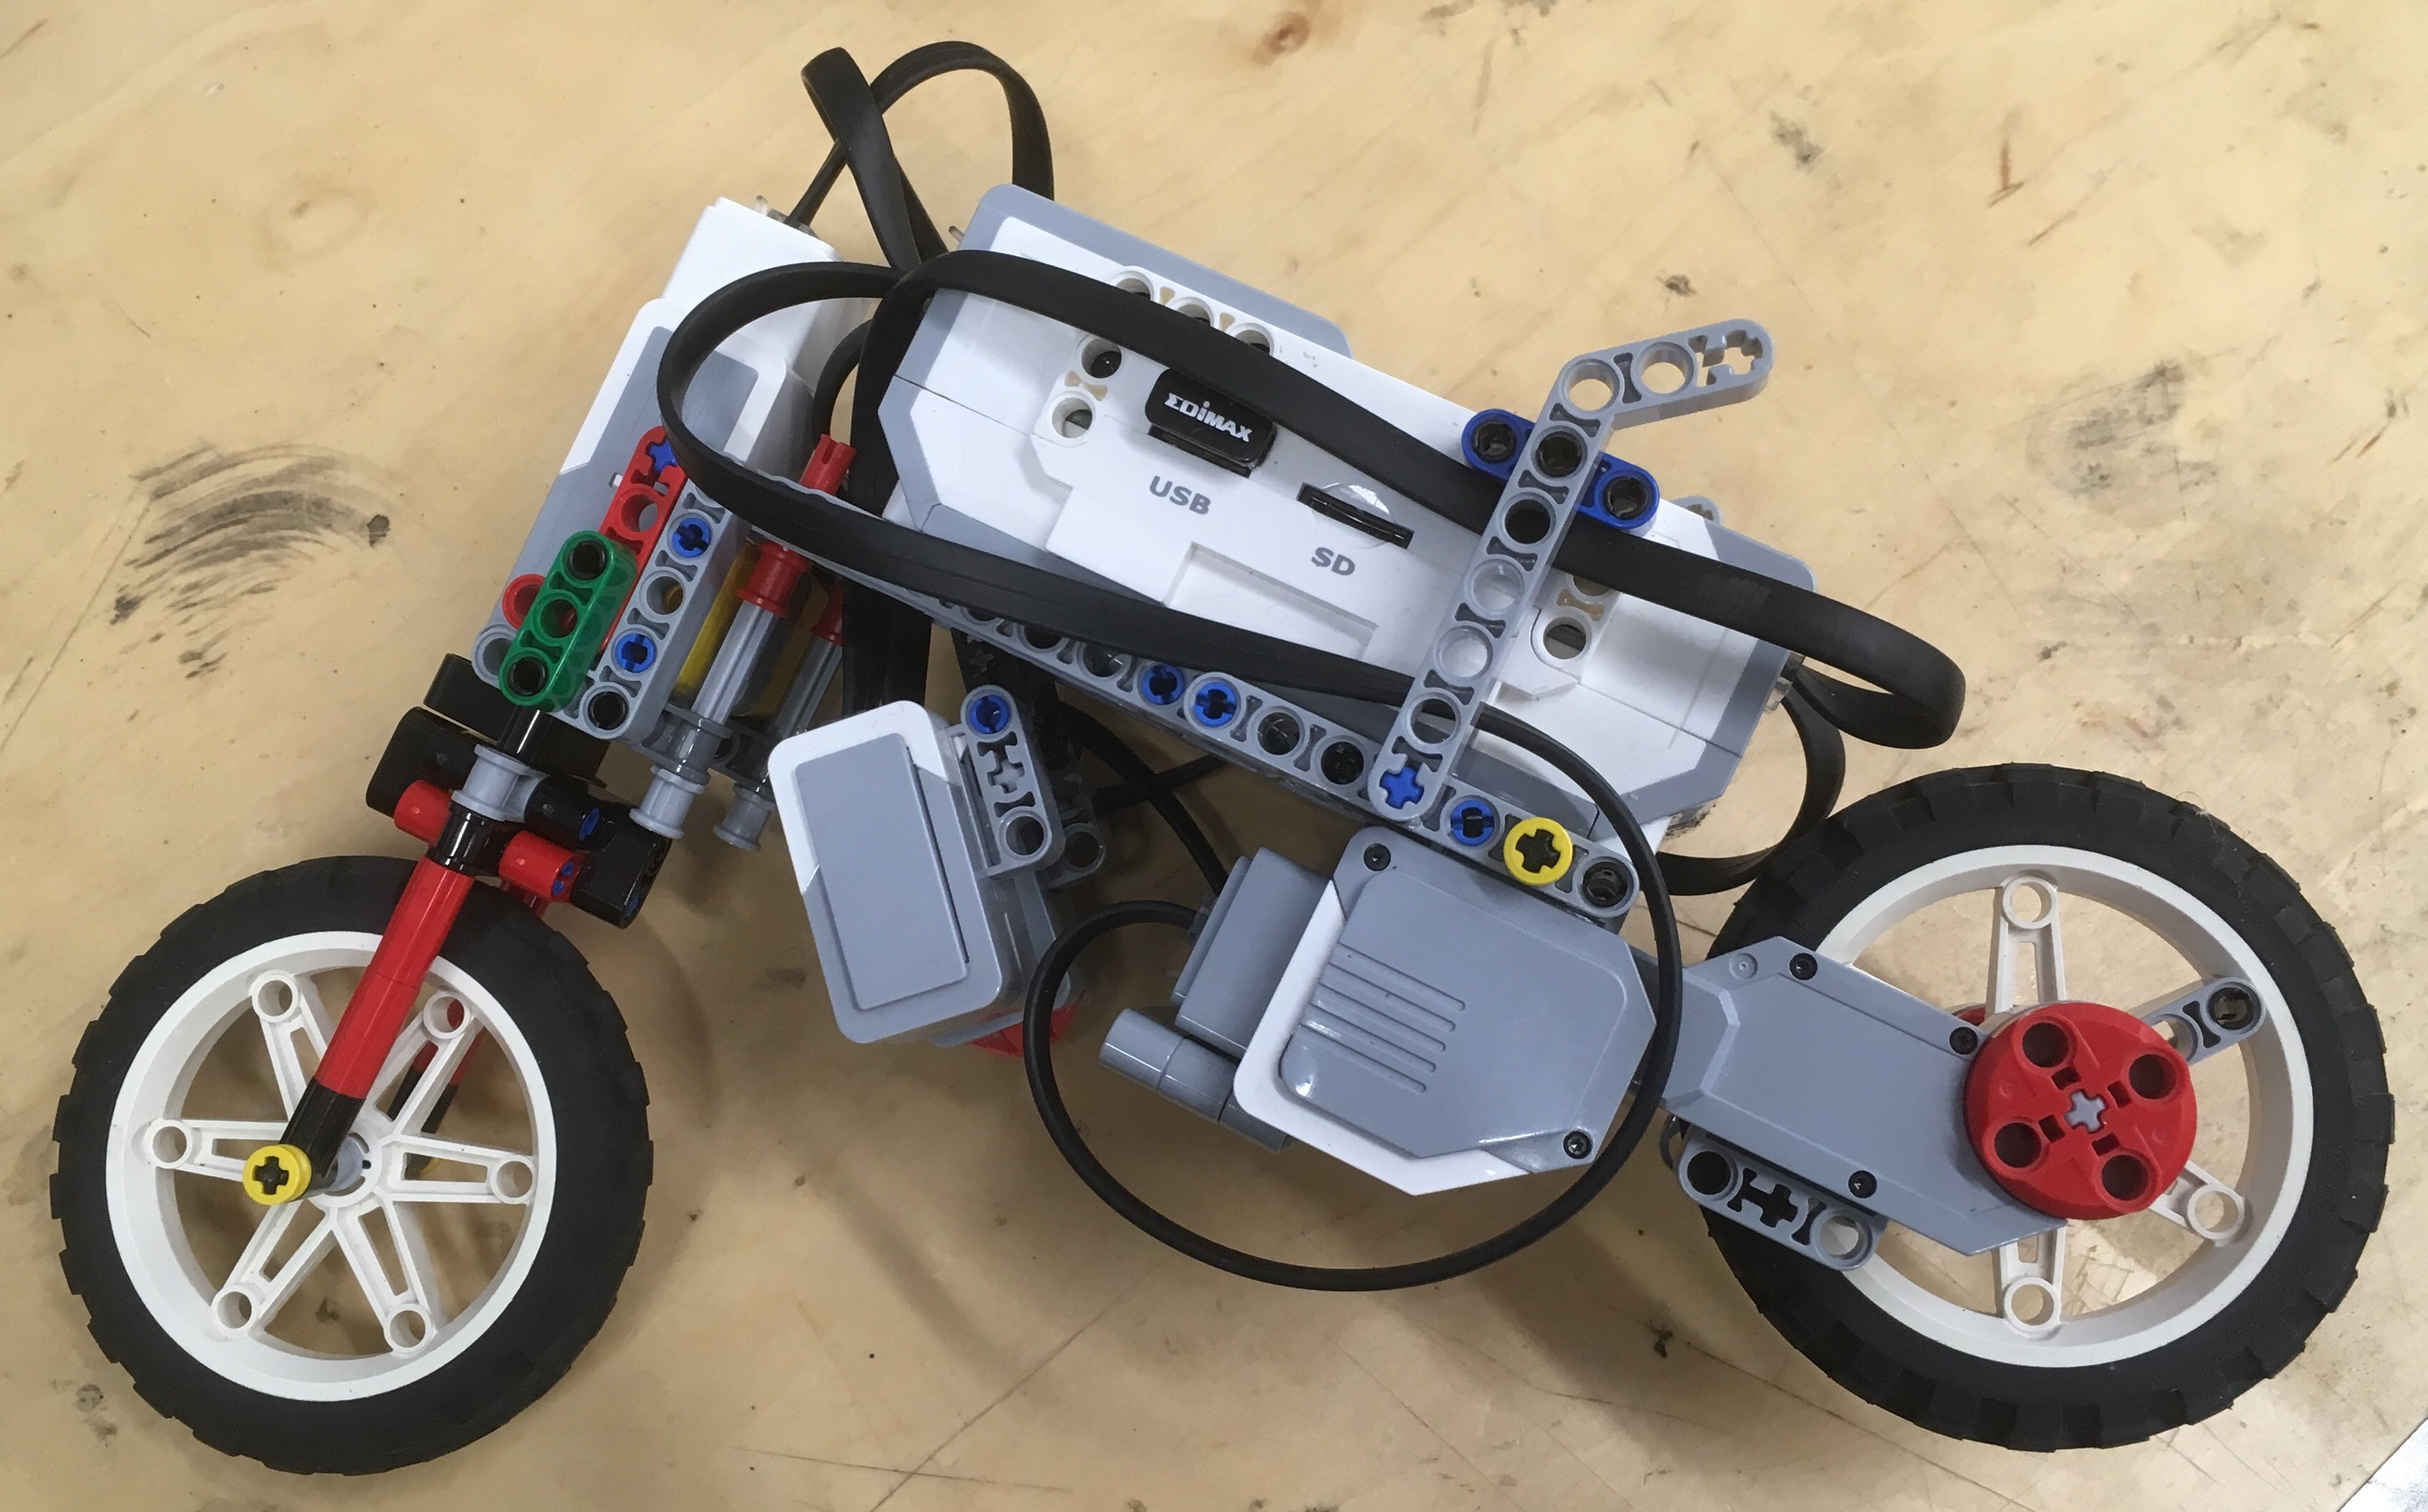
\includegraphics[scale=0.06]{LegoBike}
\caption{Lego Mindstorms Prototype Bicycle}
\end{figure}


\section{Future Work}
As detailed above, the main body of work regarding this project has been completed and a successful prototype developed. However, there are some additional items of interest that will be briefly demonstrated here, which will be worked on during Lent term.

\noindent \textbf{Improvement of Prototype} \\
A PD controller was able to stabilise the prototype bicycle. However, the gains did not match the theoretically calculated ones. Furthermore, the motion of the bicycle - although stable - was quite oscillatory. The system will be checked for modelling errors and attempts will be made to reduce the oscillations. \\

\noindent \textbf{Full-Scale Bicycle} \\
The receipt of a \textit{James Dyson IIB Project Bursary} provides the necessary funds to be able to equip a full-scale bicycle with the actuators and sensors needed to implement the control algorithms used on the smaller prototype. This will be the main focus of work during Lent term. The sourcing of components, mechanical design, and up-scaling of the control strategies are expected to prove to be difficult. \\

\noindent \textbf{Trajectory Tracking} \\
In certain situations it may be helpful to have a path-planning and following feature (such as in self-driving cars). This also provides interesting research options into topics, such as sensor fusion (GPS and IMU) and path planning. However, a stable, well-working controller is needed before this task can be addressed. 

\section*{References}

[1] "The Stability of the Motion of a Bicycle" \\
\textit{Whipple} (The Quarterly Journal of Pure and Applied Mathematics, 1899) \\

\noindent [2] "A Multibody Dynamics Benchmark on the Equations of Motion of an Uncontrolled Bicycle" \\
\textit{Schwab, Meijaard, Papadopoulos} (ENOC-2005, 2005) \\

\noindent [3] "Bicycle Dynamics and Control: Adapted bicycles for education and research" \\
\textit{Astrom, Klein, and Lennartsson} (IEEE Control Systems, 2005) \\

\noindent [4] "Virtual Model Control: An Intuitive Approach for Bipedal Locomotion" \\
\textit{Pratt, Chew, Torres, Dilworth, Pratt} (MIT, 2001) \\

\noindent [5] "Putting Energy Back in Control" \\
\textit{Ortega, van der Schaft, Mareels, Maschke} (IEEE Control Systems, 2001)

\section*{Links to Resources}

[A] Bike Simulator and Python Script Source Code: \\
\textit{https://github.com/pms67/Self-Balancing-Bike} \\

\noindent [B] Video of Lego Mindstorms Prototype \\
\textit{https://www.youtube.com/watch?v=Wknbr2rZ5ZI}

\end{document}